% Copyright 2010 Juan Rada-Vilela
% 
% Licensed under the Apache License, Version 2.0 (the "License");
% you may not use this file except in compliance with the License.
% You may obtain a copy of the License at
% 
%     http://www.apache.org/licenses/LICENSE-2.0
% 
% Unless required by applicable law or agreed to in writing, software
% distributed under the License is distributed on an "AS IS" BASIS,
% WITHOUT WARRANTIES OR CONDITIONS OF ANY KIND, either express or implied.
% See the License for the specific language governing permissions and
% limitations under the License.

\documentclass[11pt, final, a4paper, openany]{book}
\usepackage[utf8]{inputenc}
\usepackage[english]{babel}
\usepackage[top=1in,bottom=1in,left=1in,right=1in]{geometry} %Para los márgenes
\usepackage{listings}
\usepackage[usenames,dvipsnames]{color}
\usepackage{url}
\usepackage{multicol}
\usepackage{enumitem}
\usepackage{graphicx}
\usepackage{lscape}
\usepackage[colorlinks]{hyperref}
\usepackage{fancyhdr}
\usepackage{subfigure}
\usepackage{palatino}

\hypersetup{
   	pdftitle={FuzzyLite v1.5: A Fuzzy Logic Control Library written in C++},
   	pdfauthor={Juan Rada-Vilela},
   	pdfkeywords={fuzzylite, fuzzy-lite, Fuzzy Logic, Fuzzy Inference System},
   	pdfborder={000},
   	linkcolor=red,
   	anchorcolor=red,
   	citecolor=blue,
   	filecolor=red,
   	urlcolor=blue
}

\newcommand{\fl}{\texttt{FuzzyLite v1.5}}

\renewcommand{\footrulewidth}{0.4pt} 



\begin{document}
	\title{\fl\\ A Fuzzy Logic Control Library written in \texttt{C++}}
	\author{by Juan Rada-Vilela}
	\date{August, 2012}
	
	\maketitle
	\setcounter{tocdepth}{4}
	
	\tableofcontents
	\listoffigures
	\pagestyle{fancy}	

	\rfoot{\footnotesize\url{http://code.google.com/p/fuzzylite/}}
	%!TEX root = ./fuzzylite-1.01.tex
\chapter{Overview}

\section{Introduction}
\fl\ is a multiplatform, free, and open-source Fuzzy Inference System (FIS) written in C++ and released under the Apache License 2.0, which makes this software freely available for commercial and non-commercial use. The idea behind this FIS is to have a very simple and lite FIS. Simple as in simple to use, simple to understand, and simple to extend, without sacrificing performance. And lite because it requires no additional libraries more than the Standard Template Library included in the C++ Standard Library. It has an object-oriented approach and a clear separation between the headers and sources, so it is easy to extend. Furthermore, it is GUI-agnostic, meaning that the FIS does not require a GUI to run, encouraging its use as a library. Nevertheless, a Qt-based GUI is provided using \fl\ as a shared library.

\section{Features}
\begin{itemize}
	\item Linguistic terms are continuous and the following ones are available: triangular, trapezoidal, rectangular, shoulder, singleton, custom function, and compound (multiple functions).
	\item Export any fuzzy system to text using a slightly modified version of the Fuzzy Controller Language (FCL).
	\item Defuzzification using center of gravity (COG). 
	\item Mamdani rule parsing with grammar checking.
	\item Takagi Sugeno rules of any order (e.g. f(x) = (sin x) / x, f(x) = 0.5 * input-1).
	\item Weights for each rule.
	\item TNorm: minimum, product, bounded difference. 
	\item SNorm: maximum, sum, bounded sum. 
	\item Modulation: clipping, scaling. 
	\item Aggregation: maximum, sum, bounded sum.
	\item Variable sampling size for membership functions to compute area and centroid.
	\item Triangulation and Trapezoidal algorithms to compute the area and
	centroid.
	\item Hedges: not, somewhat, very, any. 
	\item Very easy to implement and incorporate new linguistic terms, defuzzification methods, fuzzy rules (antecedents and consequents), fuzzy operations (T-Norms, S-Norms, methods for modulation and aggregation), algorithms for computing the area and centroid of linguistic terms, hedges, among other things.
	
\end{itemize}

\section{What's new?}

	\subsection{\fl}
	\begin{itemize} 
	  \item Fixed the Triangulation Algorithm to include the first and last
	  triangle (improved accuracy). Courtesy of rctaylor.
	  \item Implemented the Trapezoidal Algorithm suggested by William Roeder,
	  although its accuracy is not as good as the Triangulation algorithm.
	  \item Created the scripts for building fuzzylite as static and dynamic
	  library, as well as building a demo version of it. Tested on Linux Ubuntu and
	  Mac OS X 10.5. Although the Unix version should work under Windows as well
	  using G++.
	  \item Added LeftShoulderTerm and RightShoulderTerm, just to provide a better
	  understanding when configuring the FuzzyEngine.
	  \item Changed all the \texttt{\#include <fuzzylite/?.h> for ``
	  fuzzylite/?.h''}.
	  \item Included the Trapezoidal Algorithm into the GUI.
	\end{itemize}

	\subsection{\texttt{FuzzyLite v.1.01}}
	\begin{itemize}
		\item 	The source can be built on Linux with no need to add several includes to some files. (I work on MacOSX and I did not build fuzzylite on Linux, I just assumed it would build just fine, but some includes were missing in some files. This was FIXED).
	\item Several scripts for building fuzzylite using a simple make. These scripts are created automatically by NetBeans, however, you do not need NetBeans to build fuzzylite nor the gui. The scripts are available for Linux and Mac OS X.
	\end{itemize}
	
	\subsection{\texttt{FuzzyLite v1.0}}
	\begin{itemize}
		% \item New linguistic terms available: sigmoidal, gaussian, sine and cosine functions.
		\item The GUI is working again.
		\item A class diagram of \fl.
		\item A detailed explanation of \fl.
		\item Minor changes.
	\end{itemize}

\section{What's next?}
	\begin{itemize}
	  \item Figure out why the accuracy of the Trapezoidal Algorithm is not as good
	  as the Triangulation algorithm.
		\item Fix the GUI so Takagi Sugeno rules can be tested with their respective graph.
		\item Improve the \texttt{InfixToPostfix} class so infix functions are parsed as one would normally expect.
		\item Load the fuzzy engine from text using the Fuzzy Controller Language (FCL).
		\item Include more linguistic terms (e.g. sigmoidal, gaussian, sine, cosine).
		\item Include more defuzzifiers (e.g. Right Most Maximum, Left Most Maximum, Mean Maximum).
		\item Make some functions inline to increase performance and check those that are already inline to ensure they do increase performance.
	\end{itemize}
	
	\section{Known bugs}
	\begin{itemize}
	  \item Accuracy of Trapezoidal Algorithm is not as good as Triangulation
	  Algorithm. Although I do not know whether it is a bug or a feature ;).
		\item \texttt{InfixToPostfix} conversion might not parse functions as one would normally expect. For example, $\sin (x) / x$ is \emph{not} equivalent to $(\sin x) / x$, the latter yields the result one might expect. Make sure by validating the postfix expression, or by evaluating its results.
		\item In the GUI, when using a Takagi Sugeno system, the output graphs do not work.
	\end{itemize}
	
\section{Building from source}

\subsection{\fl}
	Inside \texttt{./fuzzylite} there are 6 folders, on each there is a
	\texttt{makefile}. So all you have to do is execute from the folder the
	command \texttt{make}. The folders are described below (notice that
	\texttt{[OS]} stands for the operating system).
	\begin{itemize}	
	  \item \texttt{[OS]-demo}: Builds a demo version of \texttt{fuzzylite} which
	  can be executed later as \texttt{./fuzzylite}. It shows the results for four
	  examples of Fuzzy Engines.
	  \item \texttt{[OS]-static}: Builds the library as a static library
	  (\texttt{fuzzylite.a}).
	  \item \texttt{[OS]-shared}: Builds the library as a dynamic library
	  (\texttt{fuzzylite.so} (unix) or \texttt{fuzzylite.dylib} (mac)).
\end{itemize}

	This is a huge improvement from those really nasty NetBeans scripts. These
	scripts were automatically created by Eclipse.

\subsection{\texttt{FuzzyLite v.1.01}}

	Version 1.01 contains the following files \texttt{linux-Makefile} and \texttt{macosx-Makefile}, and the following folders \texttt{linux-nbproject} and \texttt{macosx-nbproject}. Depending on your platform, you must rename them by removing the name of the platform, so the new names are \texttt{Makefile} and \texttt{nbproject} respectively. This should work, otherwise, follow the steps below.

	\begin{enumerate}
		\item Create a \texttt{C++} Project either in Eclipse IDE or Netbeans IDE.
		\item Add all the source files and include files to the project.
		\item Add \texttt{.} to the includes path in the project properties.
		\item Add the directive \texttt{-DFL\_USE\_LOG} to enable the use of logging via \texttt{FL\_LOG(message)}. In \texttt{./include/defs.h} there are more symbols that can be defined via \texttt{-D} for further customization.
		\item Decide whether to build a library or an executable (in project properties).
		\item Use the IDE's normal build.
	\end{enumerate}

\subsection{Graphic User Interface}
	\subsection{Requirements}
	\begin{itemize}
	  \item \texttt{Qt} which can be freely downloaded from
	  \url{http://qt.nokia.com/}.
	  
\end{itemize}
	\subsection{\fl}
	In order to build this version, all you need to do (aside from having
	installed \texttt{Qt} which can be freely downloaded from
\url{http://qt.nokia.com/}.) is execute from \texttt{./fuzzylite/} the command
\texttt{qmake}. This will create a Makefile. Then, run \texttt{make} and it
should start building the GUI. Notice that in \texttt{gui.pro} it links
 to the \texttt{unix} version of \texttt{fuzzylite} static library using
 relative path, so be sure to build such library first. If it is not
 \texttt{unix} what you need, perform your changes accordingly.

	\subsection{\texttt{FuzzyLite v.1.01}}
In order to build the graphical user interface of \fl, it is necessary to first
install \texttt{Qt} which can be freely downloaded from
\url{http://qt.nokia.com/}.
	
The \texttt{Makefile} included within the \texttt{./gui} is quite easy to read.
Basically, the most important thing here is to copy the
\texttt{libfuzzylite.dylib} (or whatever the extension be according to your
platform) into the folder \texttt{./gui/dist} which is where the executable will
be put. An alternative is to copy the library into \texttt{/usr/local/lib} and
comment those lines in the \texttt{Makefile} that build and copy the library
into the \texttt{./gui/dist} directory.
	
After configuring the \texttt{Makefile} to fit your system, a \texttt{make all}
from \texttt{./gui} would build the graphical user interface of \fl. To run, it
suffices to execute \texttt{./gui} from \texttt{./gui/dist}.
	
	\section{Acknowledgements}
This work was possible thanks to the Foundation for the Advancement of Soft
Computing, to the Master of Soft Computing and Intelligent Data Analysis, and
especially to Sergio Guadarrama and Luis Magdalena.


	%!TEX root = ./fuzzylite-1.01.tex
\chapter{The Model}
	This chapter is devoted to explain \fl\ by means of a class diagram based on UML. For a better comprehension, it is divided in five groups: Fuzzy operations, Linguistic variables and terms, Linguistic terms, Fuzzy rules, Fuzzy engine, and Fuzzy exceptions. It is important to mention that all classes related to \fl\ are inside the namespace \texttt{fl}.
	
	\section{Fuzzy operations}
		Figure~\ref{f:fuzzy-ops} shows the class diagram for this group. The classes that can be seen in it are briefly explained in the following sections.
		
		\begin{landscape}
			

		\begin{figure}[ht]
			\centering
			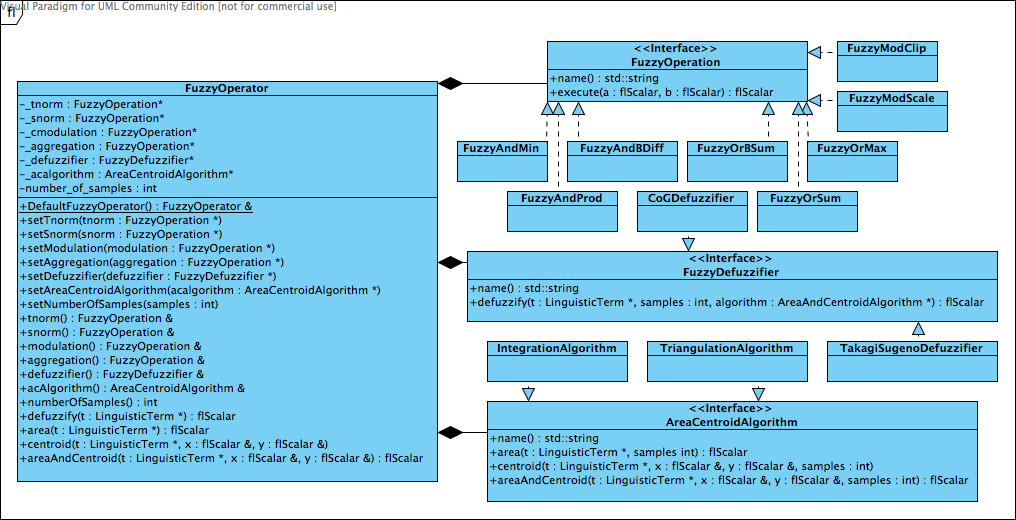
\includegraphics[scale=0.7]{./figures/fuzzy-ops.png}
			\caption{Class diagram: Fuzzy operations}
			\label{f:fuzzy-ops}
		\end{figure}
				\end{landscape}
		
		\subsection{\texttt{FuzzyOperator}}
			\texttt{FuzzyOperator} centralizes all the operations that can be performed in the fuzzy system. It contains the type of T-Norms, S-Norms, modulation, aggregation, defuzzification methods, algorithms for computing the area and centroid of any linguistic term, and the number of samples that are drawn from any linguistic term to be used by the algorithm. 
			
			This class has an static default \texttt{FuzzyOperator} instance that can be obtained using the method \texttt{fl::FuzzyOperator::DefaultFuzzyOperator()} anywhere and anytime. The defaults for this operator are the following

			\begin{multicols}{2}
			\begin{itemize}[nolistsep]
				\item \textbf{T-Norm:} \texttt{FuzzyAndMin}.
				\item \textbf{S-Norm:} \texttt{FuzzyOrMax}.
				\item \textbf{Modulation:} \texttt{FuzzyModClip}.
				\item \textbf{Aggregation:} \texttt{FuzzyOrMax}.
				\item \textbf{Defuzzifier:} \texttt{CoGDefuzzifier}.
				\item \textbf{Algorithm:} \texttt{TriangulationAlgorithm}.
				\item \textbf{Number of samples:} 100.
			\end{itemize}
			\end{multicols}
	
	These defaults may be changed at any moment from anywhere, but consider that this is an instance that is shared among all instances from many classes, so be careful about changing these values. Nevertheless, if you need to, you may use different instances among all those classes composed by \texttt{FuzzyOperator}. 
	
	\subsection{\texttt{FuzzyOperation}}
		This is the interface shared by all T-Norms, S-Norms, and methods for modulation and aggregation. If you want to implement your own operations, you may do so by implementing  this interface. The operations included in \fl\ are:
		
		\begin{itemize}
			\item T-Norm: minimum (\texttt{FuzzyAndMin}), product (\texttt{FuzzyAndProd}), and bounded difference (\texttt{FuzzyAndBDiff}).
			\item S-Norm: maximum (\texttt{FuzzyOrMax}), sum (\texttt{FuzzyOrSum}), bounded sum (\texttt{FuzzyOrBSum}).
			\item Modulation: clipping (\texttt{FuzzyModClip}), scaling (\texttt{FuzzyModScale}).
			\item Aggregation: maximum (\texttt{FuzzyOrMax}), sum (\texttt{FuzzyOrSum}), bounded sum (\texttt{FuzzyOrBSum}).
		\end{itemize}
		
	\subsection{\texttt{FuzzyDefuzzifier}}
		This is the interface shared by all defuzzifiers. If you want to implement a different defuzzifier, you may do so by implementing this interface. The defuzzifiers included in \fl\ are: Centre of Gravity (\texttt{CoGDefuzzifier}) for Mamdani rules, and \texttt{TakagiSugenoDefuzzifier} for Takagi-Sugeno rules.
		
	\subsection{\texttt{AreaAndCentroidAlgorithm}}
		This is an interface used for computing the area and centroid of linguistic terms. The algorithms included in \fl\ are: \texttt{TriangulationAlgorithm} which is a triangulation algorithm appropriate for terms that can be easily triangulated, and \texttt{IntegrationAlgorithm} which is a regular integration algorithm. The algorithm should be chosen according to the shape of the fuzzy partitions. You may also create your own algorithm by implementing this interface.
		
		
	\section{Linguistic variables and terms}
		Figure~\ref{f:linguistics} shows the class diagram for the linguistic variables and terms included in \fl. 
		
		\begin{landscape}
			

		\begin{figure}[ht]
			\centering
			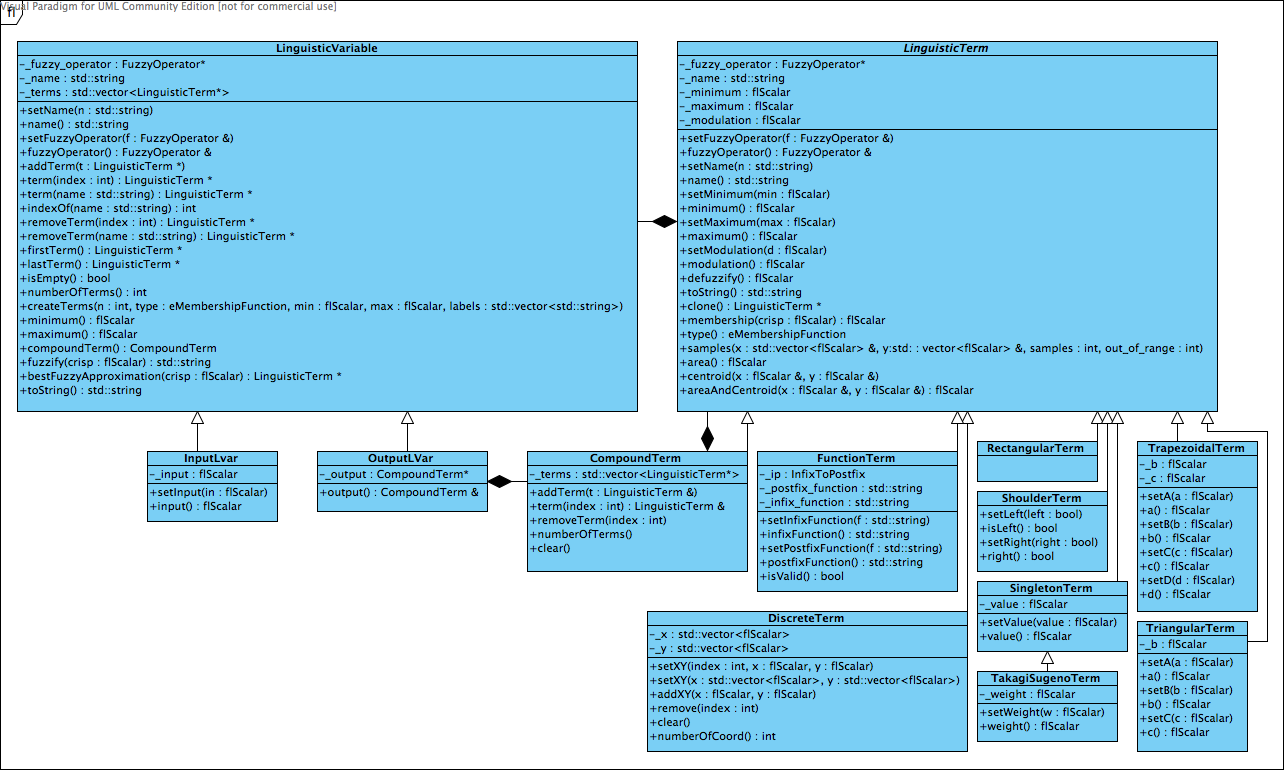
\includegraphics[scale=0.55]{./figures/fuzzy-linguistic.png}
			\caption{Class diagram: Linguistic variables and terms}
			\label{f:linguistics}
		\end{figure}
		\end{landscape}		
		\subsection{\texttt{LinguisticVariable}}
			Linguistic variables are composed of a vector of \texttt{LinguisticTerm}s. This is an abstract class that is used as base for input variables (\texttt{InputLVar}) and output variables (\texttt{OutputLVar}). Each input variable has an input value that should be the input received by the system, and each output variable has a compound linguistic term composed by all the linguistic terms added by the activation of the different rules given the input values of the input variables and their respective processing.
			
		\subsection{\texttt{LinguisticTerm}}
			Linguistic terms, also known as fuzzy partitions, define the shape of each label. Each linguistic term has a minimum and maximum that are used to define the limits of the area it covers. Several linguistic terms are included in \fl:

			\begin{itemize}
				\item \texttt{TriangularTerm}: is the well known triangular term, it is defined by its three vertices $a$, $b$, and $c$, where $a$ and $c$ are wrappers of \texttt{minimum()} and \texttt{maximum()}, respectively.
				\item \texttt{RectangularTerm}: is a simple rectangular term delimited by the minimum and maximum of its parent class \texttt{LinguisticTerm}.
				\item \texttt{TrapezoidalTerm}: defines a trapezoid by its four vertices $a$, $b$, $c$, and $d$, where $a$ and $d$ are wrappers of \texttt{minimum()} and \texttt{maximum()}, respectively.
				\item \texttt{SingletonTerm}: defines a singleton for the value $v$ delimited by $v - \delta_{low}$ and $v + \delta_{hi}$ where $\delta_{low}$ and $\delta_{hi}$ are very small values in order to be able to create samples of this term.
				\item \texttt{ShoulderTerm}: defines a trapezoid that extends to $\pm\infty$  depending on whether it is left ($-\infty$) or right ($+\infty$).
				\item \texttt{DiscreteTerm}: is a term composed of a vector of $(x,y)$ coordinates.  It is important to note that when sampling this type of term, the result of \texttt{membership(flScalar crisp)} is the value of $y$ for the closest $x$ given the value of \texttt{crisp}.
				\item \texttt{FunctionTerm}: is a term that is defined as a function $f(x)$ which accepts several mathematical and trigonometrical operations over a given function, for example: \texttt{setInfixFunction( "(sin x) / x" )}. It is \emph{very} important to remark that the parser used to parse infix functions may not function as expected (e.g. $\sin (x) / x$ is different of $(\sin x) / x$, the latter one gives the result one expects). When in doubt, test your expression by converting it to postfix.
				\item \texttt{CompoundTerm}: is a term composed of a list of \texttt{LinguisticTerm}s. This is used in \texttt{OutputLVar} in order to aggregate all the linguistic terms that were added by the activation of rules, but it may be used as well to create more complex partitions.
				\item \texttt{TakagiSugenoTerm}: is a term used when dealing with \texttt{TakagiSugenoRule}s, it extends from \texttt{SingletonTerm} so it has a value, and it  includes a \texttt{weight} as well, both necessary for this kind of system.
			\end{itemize}

			Finally, figure~\ref{f:lterms} shows examples of the linguistic terms, obtained by printing the window from the GUI developed for \fl.

		\begin{figure}[ht]
			\centering
			\subfigure[\texttt{TriangularTerm}] 
			{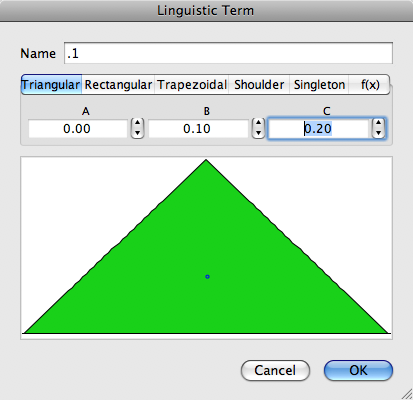
\includegraphics[scale=0.3]
			{./figures/ft-triangular.png}} 
			\subfigure[\texttt{RectangularTerm}]
			{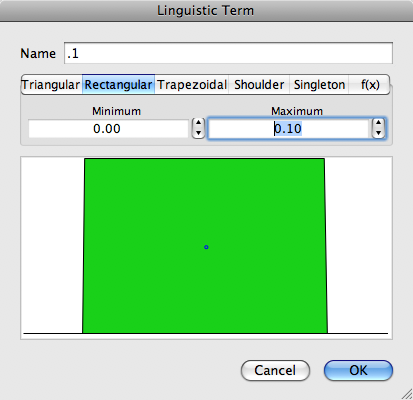
\includegraphics[scale=0.3]
			{./figures/ft-rectangular.png}}
			\subfigure[\texttt{TrapezoidalTerm}]
			{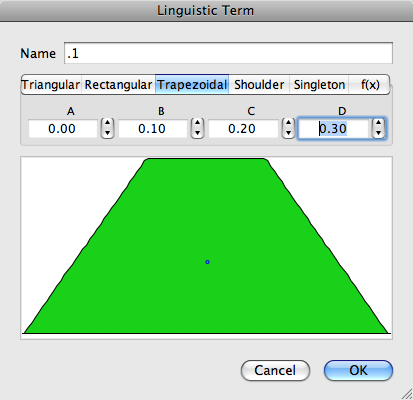
\includegraphics[scale=0.3]
			{./figures/ft-trapezoidal.png}} \\
			\subfigure[\texttt{SingletonTerm}]
			{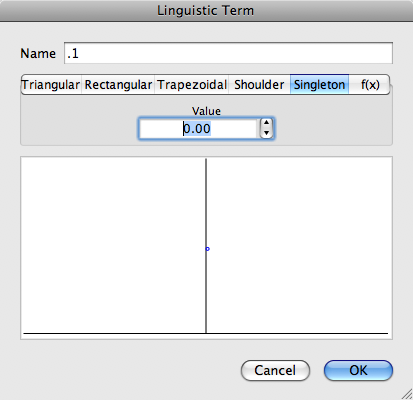
\includegraphics[scale=0.3]
			{./figures/ft-singleton.png}} 
			\subfigure[\texttt{ShoulderTerm} (left)] 
			{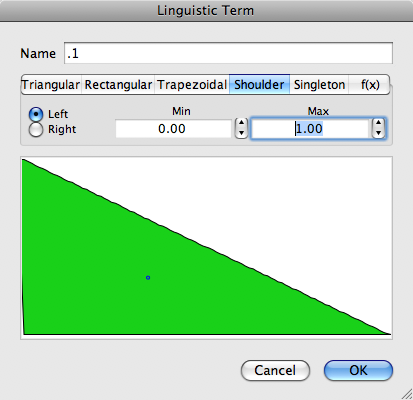
\includegraphics[scale=0.3]
			{./figures/ft-lshoulder.png}} 
			\subfigure[\texttt{ShoulderTerm} (right)]
			{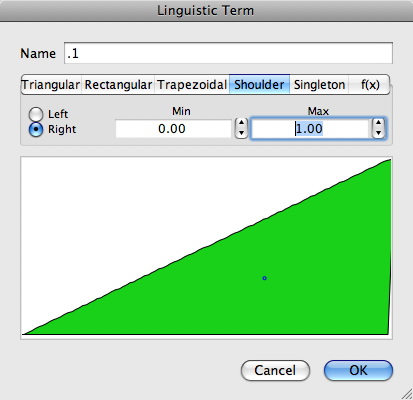
\includegraphics[scale=0.3]
			{./figures/ft-rshoulder.png}}\\
			\subfigure[\texttt{FunctionTerm}]
			{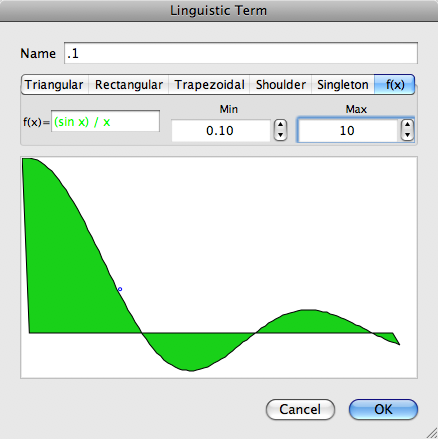
\includegraphics[scale=0.3]
			{./figures/ft-function.png}}
			\subfigure[Triangular partitions]
			{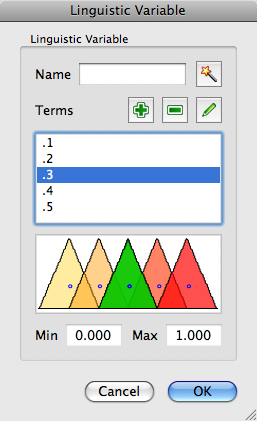
\includegraphics[scale=0.4]
			{./figures/ft-partition-1.png}}
			\subfigure[Triangular + Shoulder partitions]
			{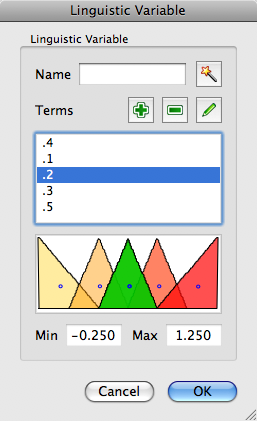
\includegraphics[scale=0.4]
			{./figures/ft-partition-2.png}}
			\caption{Linguistic Terms}
			\label{f:lterms}
		\end{figure}
		
	\section{Fuzzy rules}
		Figure~\ref{f:fuzzy-rules} shows the class diagram for fuzzy rules and all its related classes included in \fl.
		
		\begin{landscape}
			\begin{figure}[ht]
				\centering
				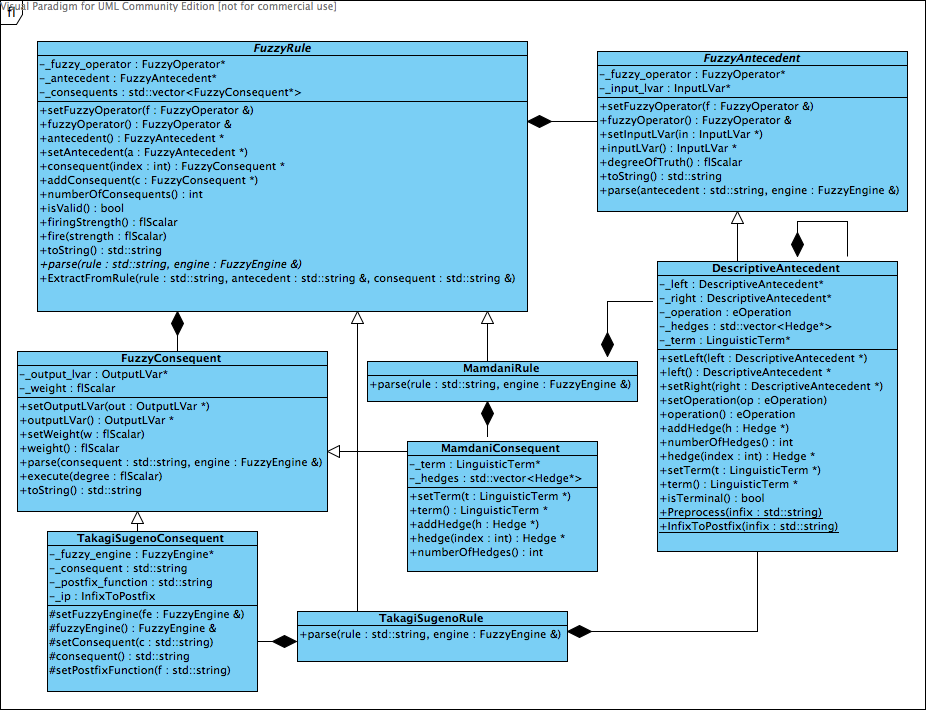
\includegraphics[scale=0.58]{./figures/fuzzy-rules.png}
				\caption{Class diagram: Fuzzy rules}
				\label{f:fuzzy-rules}
			\end{figure}
		\end{landscape}
		
		\subsection{\texttt{FuzzyRule}}
			This abstract class is the base for \texttt{MamdaniRule}s and \texttt{TakagiSugenoRule}s. It is composed by an antecedent (\texttt{FuzzyAntecedent}) and a list of consequents (\texttt{FuzzyConsequent}s). There are two methods that are worth mentioning here: \texttt{firingStrength()} which determines the activation degree of the rule given the inputs in the \texttt{InputLVar}s, and \texttt{fire( flScalar d )} which fires the rule with a degree $d$. When firing the rule, the consequents are modulated according to $d$ and then added to the \texttt{OutputLVar}s with the respective weight of the rule. It is also important to remark that parsing the rules is case-sensitive.
			
		\subsubsection{\texttt{FuzzyAntecedent} and \texttt{FuzzyConsequent}}
			These abstract classes represent the antecedent and consequent of a rule, respectively. \texttt{FuzzyAntecedent} has a pointer to the input variable to which it is related in order to access the value of the respective \texttt{InputLVar}, similarly, \texttt{FuzzyConsequent} has a pointer to the output variable to which it is related in order to aggregate the respective modulated linguistic term to the output.
			
			
		\subsubsection{\texttt{DescriptiveAntecedent}}
			This class is based on \texttt{FuzzyAntecedent} and it is a red-black tree that relates two propositions with an operator, for example, \texttt{input-1} \textbf{is} \texttt{LOW} \textbf{and}  \texttt{input-2} \textbf{is} \texttt{GOOD} is separated into a left antecedent (\texttt{input-1} \textbf{is} \texttt{LOW}), an operator (\textbf{and}),   and a right antecedent (\texttt{input-2} \textbf{is} \texttt{GOOD}). Given the recursion of  this model, it is possible to create rules of any depth, as it is evaluated bottom-up. This is the class used by \texttt{MamdaniRule} and \texttt{TakagiSugenoRule}.
		
		\subsubsection{\texttt{Hedge}}
			Hedges are modifiers of the propositions (antecedent) and actions (consequent). All hedges must implement the interface \texttt{Hedge}, and must be included when configuring the \texttt{FuzzyEngine}. \fl\ includes four hedges: not (\texttt{HedgeNot}), somewhat (\texttt{HedgeSomewhat}), very (\texttt{HedgeVery}), any (\texttt{HedgeAny}). In order to use \texttt{HedgeAny}, it is necessary to include a \emph{dummy} linguistic term to comply with the general form of the rules (i.e. \emph{input-1} \textbf{is} \texttt{any} \texttt{LOW}); this hedge will always return 1.0, so it does not matter the linguistic term as long as it is within the linguistic variable used. Figure~\ref{f:hedges} shows the class diagram regarding hedges.
			
			\begin{figure}[ht]
				\centering
				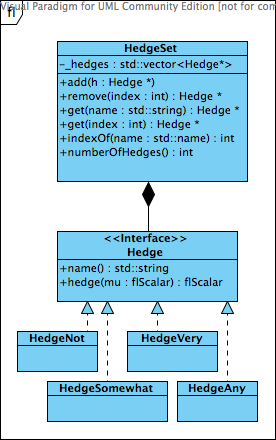
\includegraphics[scale=0.65]{./figures/fuzzy-hedges.png}
				\caption{Class diagram: Hedges}
				\label{f:hedges}
			\end{figure}
		
		\subsubsection{\texttt{MamdaniRule} and \texttt{TakagiSugenoRule}}
			These classes represents the type of rules of a system based on Mamdani's rules, and the one based on Takagi-Sugeno rules, respectively. They extend the abstract class \texttt{FuzzyRule} by implementing the \texttt{parse()} method accordingly. Both classes use \texttt{DescriptiveAntecedent} as the antecedent of the rule, but differ in the consequent: \texttt{MamdaniRule} uses \texttt{MamdaniConsequent}, and \texttt{TakagiSugenoRule} uses \texttt{TakagiSugenoConsequent}.
			
		\subsubsection{\texttt{MamdaniConsequent} and \texttt{TakagiSugenoConsequent}}
			The consequent of a Mamdani rule is of the form: \texttt{OutputLVar} \textbf{is} [\texttt{Hedge}$^*$] \texttt{LinguisticTerm}, where [\texttt{Hedge}$^*$] means that none or many hedges may be included.
			
			Conversely, the consequent of a Takagi-Sugeno rule is of the form \texttt{OutputLVar}=\{\emph{expression}\}, where \emph{expression} is a mathematical expression that may include references to the values of the \texttt{InputLVar}s, in which case the name of the input variable is used (e.g. "... f\_x=0.5 * input-1 + (sin input-2)"). This implementation also allows to include previously computed outputs, in which case the name of the output should be used instead.
	
	\section{Fuzzy engine}
		The class diagram for this group can be seen in figure~\ref{f:fuzzy-engine}. It contains the class \texttt{FuzzyEngine} which is composed by a \texttt{FuzzyOperator}, a vector of \texttt{RuleBlock}s which contain the \texttt{FuzzyRule}s, a \texttt{HedgeSet} that contains the hedges registered in the engine, and a vector of \texttt{InputLVar}s and \texttt{OutputLVar}s for input and output variables (respectively).
		
		The \texttt{FuzzyEngine} class contains the whole fuzzy control system. The only methods which might require a bit of explanation are \texttt{process( bool )}, and \texttt{process(int, bool)}. The former receives a boolean parameter that defaults to \texttt{true} and (if true) clears the output of all the output variables. The latter receives an \texttt{int} parameter that determines the index of the \texttt{RuleBlock} to be fired, and a \texttt{bool} that defaults to \texttt{true} which defines whether to clear the output of the output variables.
		
		\begin{landscape}
		\begin{figure}[ht]
			\centering
			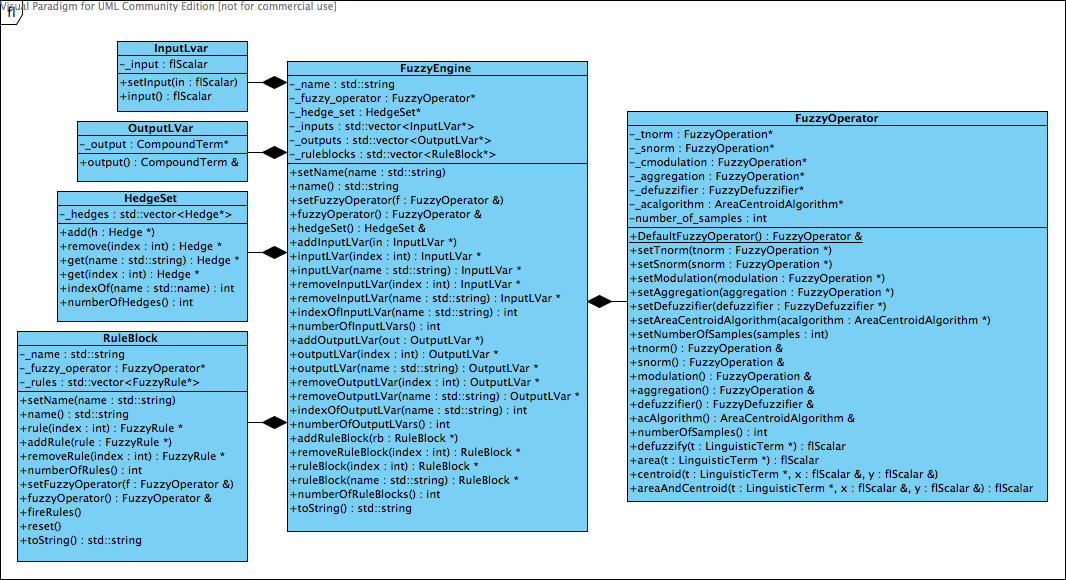
\includegraphics[scale=0.65]{./figures/fuzzy-engine.png}
			\caption{Class diagram: Fuzzy engine}
			\label{f:fuzzy-engine}
		\end{figure}
		\end{landscape}
	
	\section{Fuzzy exceptions}
		This group contains some exceptions that are used within several classes of \fl. The class \texttt{FuzzyException} extends the \texttt{std::exception} of the Standard Template Library (STL), and adds additional methods. The other classes derived from \texttt{FuzzyException} also contain some static methods to help a bit with the programming. There is not much to say about these exceptions, except to take a look at the code when using them to become familiar. Figure~\ref{f:fuzzy-exceptions} shows the class diagram for this group.
		
		
	\begin{figure}[ht]
		\centering
		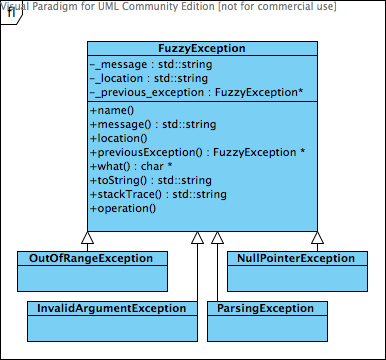
\includegraphics[scale=0.65]{./figures/fuzzy-exceptions.png}
		\caption{Class diagram: Fuzzy exceptions}
		\label{f:fuzzy-exceptions}
	\end{figure}
	
	

	%!TEX root = ./fuzzylite-1.01.tex
	\chapter{Examples}
	\section{Example \#1: Basic FIS}
		This is a basic FIS composed of one input variable and one output variable.
	\lstset{language=[ISO]C++, texcl=true,
	numbers=left, numberstyle=\tiny, stepnumber=1, numbersep=5pt,basicstyle=\footnotesize\tt,keywordstyle=\color{Purple}\bfseries, 
	stringstyle=\color{RoyalBlue}, % typewriter type for strings 
	showstringspaces=false,
	classoffset=1,
	morekeywords={*}, keywordstyle=\color{red},
	classoffset=0}
	
	\begin{lstlisting}[firstnumber=1,tabsize=2]
	fl::FuzzyEngine engine;
	engine.hedgeSet().add(new fl::HedgeNot);
	engine.hedgeSet().add(new fl::HedgeSomewhat);
	engine.hedgeSet().add(new fl::HedgeVery);
	fl::InputLVar* energy = new fl::InputLVar("Energy");
	energy->addTerm(new fl::ShoulderTerm("LOW", 0.25, 0.5, true));
	energy->addTerm(new fl::TriangularTerm("MEDIUM", 0.25, 0.75));
	energy->addTerm(new fl::ShoulderTerm("HIGH", 0.50, 0.75, false));
	engine.addInputLVar(energy);

	fl::OutputLVar* health = new fl::OutputLVar("Health");
	health->addTerm(new fl::TriangularTerm("BAD", 0.0, 0.50));
	health->addTerm(new fl::TriangularTerm("REGULAR", 0.25, 0.75));
	health->addTerm(new fl::TriangularTerm("GOOD", 0.50, 1.00));
	engine.addOutputLVar(health);
	fl::RuleBlock* block = new fl::RuleBlock();
	block->addRule(new fl::MamdaniRule("if Energy is LOW then Health is BAD", engine));
	block->addRule(new fl::MamdaniRule("if Energy is MEDIUM then Health is REGULAR", engine));
	block->addRule(new fl::MamdaniRule("if Energy is HIGH then Health is GOOD", engine));
	engine.addRuleBlock(block);

	\end{lstlisting}
	
	Once the FIS is configured, the control process may begin anytime by setting the input value to the input variables and processing. For example,
	
	\begin{lstlisting}[firstnumber=last,tabsize=2]
	for (fl::flScalar in = 0.0; in < 1.1; in += 0.1) {
	    energy->setInput(in);
	    engine.process();
	    fl::flScalar out = health->output().defuzzify();
	    FL_LOG("Energy=" << in);
	    FL_LOG("Energy is " << energy->fuzzify(in));
	    FL_LOG("Health=" << out);
	    FL_LOG("Health is " << health->fuzzify(out));
	    FL_LOG("--");
	}
	\end{lstlisting}
	
	The previous code would yield the following results in console (assuming that \texttt{FL\_USE\_LOG} was defined):
	
	\begin{lstlisting}
Energy=0
Energy is 1.000/LOW + 0.000/MEDIUM + 0.000/HIGH
Health=0.249902
Health is 1.000/BAD + 0.000/REGULAR + 0.000/GOOD
--
Energy=0.1
Energy is 1.000/LOW + 0.000/MEDIUM + 0.000/HIGH
Health=0.249902
Health is 1.000/BAD + 0.000/REGULAR + 0.000/GOOD
--
Energy=0.2
Energy is 1.000/LOW + 0.000/MEDIUM + 0.000/HIGH
Health=0.249902
Health is 1.000/BAD + 0.000/REGULAR + 0.000/GOOD
--
Energy=0.3
Energy is 0.800/LOW + 0.200/MEDIUM + 0.000/HIGH
Health=0.309985
Health is 0.760/BAD + 0.240/REGULAR + 0.000/GOOD
--
Energy=0.4
Energy is 0.400/LOW + 0.600/MEDIUM + 0.000/HIGH
Health=0.394929
Health is 0.420/BAD + 0.580/REGULAR + 0.000/GOOD
--
Energy=0.5
Energy is 0.000/LOW + 1.000/MEDIUM + 0.000/HIGH
Health=0.499902
Health is 0.000/BAD + 1.000/REGULAR + 0.000/GOOD
--
Energy=0.6
Energy is 0.000/LOW + 0.600/MEDIUM + 0.400/HIGH
Health=0.604537
Health is 0.000/BAD + 0.582/REGULAR + 0.418/GOOD
--
Energy=0.7
Energy is 0.000/LOW + 0.200/MEDIUM + 0.800/HIGH
Health=0.689444
Health is 0.000/BAD + 0.242/REGULAR + 0.758/GOOD
--
Energy=0.8
Energy is 0.000/LOW + 0.000/MEDIUM + 1.000/HIGH
Health=0.749902
Health is 0.000/BAD + 0.000/REGULAR + 1.000/GOOD
--
Energy=0.9
Energy is 0.000/LOW + 0.000/MEDIUM + 1.000/HIGH
Health=0.749902
Health is 0.000/BAD + 0.000/REGULAR + 1.000/GOOD
--
Energy=1
Energy is 0.000/LOW + 0.000/MEDIUM + 1.000/HIGH
Health=0.749902
Health is 0.000/BAD + 0.000/REGULAR + 1.000/GOOD
--
	\end{lstlisting}
	
	\section{Example \#2: 3D Pole Balancing}
		A simulation video of this fuzzy system implemented with \fl\ as shown below is available at \url{http://www.youtube.com/watch?v=YOKk8G_5aRA}.
	\lstset{language=[ISO]C++, texcl=true,
	numbers=left, numberstyle=\tiny, stepnumber=1, numbersep=5pt,basicstyle=\footnotesize\tt,keywordstyle=\color{Purple}\bfseries, 
	stringstyle=\color{RoyalBlue}, % typewriter type for strings 
	showstringspaces=false,
	classoffset=1,
	morekeywords={*}, keywordstyle=\color{red},
	classoffset=0}
	
	\begin{lstlisting}[firstnumber=1,tabsize=2]
FuzzyEngine engine("pole-balancing-3d");

InputLVar* anglex = new InputLVar("AngleX");
std::vector<std::string> labels;
labels.push_back("NEAR_0");
labels.push_back("NEAR_45");
labels.push_back("NEAR_90");
labels.push_back("NEAR_135");
labels.push_back("NEAR_180");
anglex->createTerms(5, LinguisticTerm::MF_SHOULDER, 0, 180, labels);
engine.addInputLVar(anglex);

InputLVar* anglez = new InputLVar("AngleZ");
labels.clear();
labels.push_back("NEAR_0");
labels.push_back("NEAR_45");
labels.push_back("NEAR_90");
labels.push_back("NEAR_135");
labels.push_back("NEAR_180");
anglez->createTerms(5, LinguisticTerm::MF_SHOULDER, 0, 180, labels);
engine.addInputLVar(anglez);

OutputLVar* forcex = new OutputLVar("ForceX");
labels.clear();
labels.push_back("NL");
labels.push_back("NS");
labels.push_back("ZR");
labels.push_back("PS");
labels.push_back("PL");
forcex->createTerms(5, LinguisticTerm::MF_TRIANGULAR, -1, 1, labels);
engine.addOutputLVar(forcex);

OutputLVar* forcez = new OutputLVar("ForceZ");
labels.clear();
labels.push_back("NL");
labels.push_back("NS");
labels.push_back("ZR");
labels.push_back("PS");
labels.push_back("PL");
forcez->createTerms(5, LinguisticTerm::MF_TRIANGULAR, -1, 1, labels);
engine.addOutputLVar(forcez);

RuleBlock* ruleblock = new RuleBlock("Rules");
ruleblock->addRule(new MamdaniRule("if AngleX is NEAR_180 then ForceX is NL", engine));
ruleblock->addRule(new MamdaniRule("if AngleX is NEAR_135 then ForceX is NS", engine));
ruleblock->addRule(new MamdaniRule("if AngleX is NEAR_90 then ForceX is ZR", engine));
ruleblock->addRule(new MamdaniRule("if AngleX is NEAR_45 then ForceX is PS", engine));
ruleblock->addRule(new MamdaniRule("if AngleX is NEAR_0 then ForceX is PL", engine));

ruleblock->addRule(new MamdaniRule("if AngleZ is NEAR_180 then ForceZ is NL", engine));
ruleblock->addRule(new MamdaniRule("if AngleZ is NEAR_135 then ForceZ is NS", engine));
ruleblock->addRule(new MamdaniRule("if AngleZ is NEAR_90 then ForceZ is ZR", engine));
ruleblock->addRule(new MamdaniRule("if AngleZ is NEAR_45 then ForceZ is PS", engine));
ruleblock->addRule(new MamdaniRule("if AngleZ is NEAR_0 then ForceZ is PL", engine));
engine.addRuleBlock(ruleblock);

FL_LOG(engine.toString());
	\end{lstlisting}

	The output from the previous block of code exports the fuzzy system to text using the Fuzzy Controller Language (FCL) as shown below. 
	
	\begin{lstlisting}
FUNCTION_BLOCK pole-balancing-3d

VAR_INPUT
AngleX: REAL;
AngleZ: REAL;
END_VAR

FUZZIFY AngleX
TERM NEAR_0 := Shoulder left(0 60);
TERM NEAR_45 := Triangular (30 60 90);
TERM NEAR_90 := Triangular (60 90 120);
TERM NEAR_135 := Triangular (90 120 150);
TERM NEAR_180 := Shoulder right(120 180);
END_FUZZIFY

FUZZIFY AngleZ
TERM NEAR_0 := Shoulder left(0 60);
TERM NEAR_45 := Triangular (30 60 90);
TERM NEAR_90 := Triangular (60 90 120);
TERM NEAR_135 := Triangular (90 120 150);
TERM NEAR_180 := Shoulder right(120 180);
END_FUZZIFY

VAR_OUTPUT
ForceX: REAL
ForceZ: REAL
END_VAR

DEFUZZIFY ForceX
TERM NL := Triangular (-1 -0.666667 -0.333333);
TERM NS := Triangular (-0.666667 -0.333333 5.96046e-08);
TERM ZR := Triangular (-0.333333 5.96046e-08 0.333333);
TERM PS := Triangular (5.96046e-08 0.333333 0.666667);
TERM PL := Triangular (0.333333 0.666667 1);
END_DEFUZZIFY

DEFUZZIFY ForceZ
TERM NL := Triangular (-1 -0.666667 -0.333333);
TERM NS := Triangular (-0.666667 -0.333333 5.96046e-08);
TERM ZR := Triangular (-0.333333 5.96046e-08 0.333333);
TERM PS := Triangular (5.96046e-08 0.333333 0.666667);
TERM PL := Triangular (0.333333 0.666667 1);
END_DEFUZZIFY

RULEBLOCK Rules
RULE 1: if AngleX is NEAR_180 then ForceX is NL;
RULE 2: if AngleX is NEAR_135 then ForceX is NS;
RULE 3: if AngleX is NEAR_90 then ForceX is ZR;
RULE 4: if AngleX is NEAR_45 then ForceX is PS;
RULE 5: if AngleX is NEAR_0 then ForceX is PL;
RULE 6: if AngleZ is NEAR_180 then ForceZ is NL;
RULE 7: if AngleZ is NEAR_135 then ForceZ is NS;
RULE 8: if AngleZ is NEAR_90 then ForceZ is ZR;
RULE 9: if AngleZ is NEAR_45 then ForceZ is PS;
RULE 10: if AngleZ is NEAR_0 then ForceZ is PL;
END_RULEBLOCK

END_FUNCTION_BLOCK		
	\end{lstlisting}

	\section{Example 3: Approximating a function}
	It is also possible to create a fuzzy system to approximate a function. For example, if we were to approximate the function $sin (x) / x$, we could do so by using the  with the following code.
	
	\lstset{language=[ISO]C++, texcl=true,
	numbers=left, numberstyle=\tiny, stepnumber=1, numbersep=5pt,basicstyle=\footnotesize\tt,keywordstyle=\color{Purple}\bfseries, 
	stringstyle=\color{RoyalBlue}, % typewriter type for strings 
	showstringspaces=false,
	classoffset=1,
	morekeywords={*}, keywordstyle=\color{red},
	classoffset=0}
	
	\begin{lstlisting}[firstnumber=1,tabsize=2]
FuzzyOperator& op = FuzzyOperator::DefaultFuzzyOperator();
op.setDefuzzifier(new TakagiSugenoDefuzzifier);
FuzzyEngine engine("approximation", op);

fl::InputLVar* x = new fl::InputLVar("x");
x->addTerm(new fl::TriangularTerm("NEAR_1", 0, 2));
x->addTerm(new fl::TriangularTerm("NEAR_2", 1, 3));
x->addTerm(new fl::TriangularTerm("NEAR_3", 2, 4));
x->addTerm(new fl::TriangularTerm("NEAR_4", 3, 5));
x->addTerm(new fl::TriangularTerm("NEAR_5", 4, 6));
x->addTerm(new fl::TriangularTerm("NEAR_6", 5, 7));
x->addTerm(new fl::TriangularTerm("NEAR_7", 6, 8));
x->addTerm(new fl::TriangularTerm("NEAR_8", 7, 9));
x->addTerm(new fl::TriangularTerm("NEAR_9", 8, 10));
engine.addInputLVar(x);

fl::OutputLVar* f_x = new fl::OutputLVar("f_x");
f_x->addTerm(new fl::FunctionTerm("function", "(sin x) / x", 0, 10));
engine.addOutputLVar(f_x);

fl::RuleBlock* block = new fl::RuleBlock();
block->addRule(new fl::TakagiSugenoRule("if x is NEAR_1 then f_x=0.84", engine));
block->addRule(new fl::TakagiSugenoRule("if x is NEAR_2 then f_x=0.45", engine));
block->addRule(new fl::TakagiSugenoRule("if x is NEAR_3 then f_x=0.04", engine));
block->addRule(new fl::TakagiSugenoRule("if x is NEAR_4 then f_x=-0.18", engine));
block->addRule(new fl::TakagiSugenoRule("if x is NEAR_5 then f_x=-0.19", engine));
block->addRule(new fl::TakagiSugenoRule("if x is NEAR_6 then f_x=-0.04", engine));
block->addRule(new fl::TakagiSugenoRule("if x is NEAR_7 then f_x=0.09", engine));
block->addRule(new fl::TakagiSugenoRule("if x is NEAR_8 then f_x=0.12", engine));
block->addRule(new fl::TakagiSugenoRule("if x is NEAR_9 then f_x=0.04", engine));

engine.addRuleBlock(block);

int n = 40;
flScalar mse = 0;
for (fl::flScalar in = x->minimum(); in < x->maximum() ;
        in += (x->minimum() + x->maximum()) / n) {
    x->setInput(in);
    engine.process();
    flScalar expected = f_x->term(0)->membership(in);
    flScalar obtained = f_x->output().defuzzify();
    flScalar se = (expected - obtained) * (expected - obtained);
    mse += isnan(se) ? 0 : se;
    FL_LOG("x=" << in << "\texpected_out=" << expected << "\tobtained_out=" << obtained
            << "\tse=" << se);
}
FL_LOG("MSE=" << mse / n);
	\end{lstlisting} 
	
	The output of this piece of code is the following.
\begin{verbatim}
x=0.000        expected_out=nan        obtained_out=nan        se=nan
x=0.250        expected_out=0.990        obtained_out=0.840        se=0.022
x=0.500        expected_out=0.959        obtained_out=0.840        se=0.014
x=0.750        expected_out=0.909        obtained_out=0.840        se=0.005
x=1.000        expected_out=0.841        obtained_out=0.840        se=0.000
x=1.250        expected_out=0.759        obtained_out=0.743        se=0.000
x=1.500        expected_out=0.665        obtained_out=0.645        se=0.000
x=1.750        expected_out=0.562        obtained_out=0.547        se=0.000
x=2.000        expected_out=0.455        obtained_out=0.450        se=0.000
x=2.250        expected_out=0.346        obtained_out=0.347        se=0.000
x=2.500        expected_out=0.239        obtained_out=0.245        se=0.000
x=2.750        expected_out=0.139        obtained_out=0.142        se=0.000
x=3.000        expected_out=0.047        obtained_out=0.040        se=0.000
x=3.250        expected_out=-0.033        obtained_out=-0.015        se=0.000
x=3.500        expected_out=-0.100        obtained_out=-0.070        se=0.001
x=3.750        expected_out=-0.152        obtained_out=-0.125        se=0.001
x=4.000        expected_out=-0.189        obtained_out=-0.180        se=0.000
x=4.250        expected_out=-0.211        obtained_out=-0.183        se=0.001
x=4.500        expected_out=-0.217        obtained_out=-0.185        se=0.001
x=4.750        expected_out=-0.210        obtained_out=-0.188        se=0.001
x=5.000        expected_out=-0.192        obtained_out=-0.190        se=0.000
x=5.250        expected_out=-0.164        obtained_out=-0.153        se=0.000
x=5.500        expected_out=-0.128        obtained_out=-0.115        se=0.000
x=5.750        expected_out=-0.088        obtained_out=-0.078        se=0.000
x=6.000        expected_out=-0.047        obtained_out=-0.040        se=0.000
x=6.250        expected_out=-0.005        obtained_out=-0.007        se=0.000
x=6.500        expected_out=0.033        obtained_out=0.025        se=0.000
x=6.750        expected_out=0.067        obtained_out=0.058        se=0.000
x=7.000        expected_out=0.094        obtained_out=0.090        se=0.000
x=7.250        expected_out=0.114        obtained_out=0.098        se=0.000
x=7.500        expected_out=0.125        obtained_out=0.105        se=0.000
x=7.750        expected_out=0.128        obtained_out=0.112        se=0.000
x=8.000        expected_out=0.124        obtained_out=0.120        se=0.000
x=8.250        expected_out=0.112        obtained_out=0.100        se=0.000
x=8.500        expected_out=0.094        obtained_out=0.080        se=0.000
x=8.750        expected_out=0.071        obtained_out=0.060        se=0.000
x=9.000        expected_out=0.046        obtained_out=0.040        se=0.000
x=9.250        expected_out=0.019        obtained_out=0.040        se=0.000
x=9.500        expected_out=-0.008        obtained_out=0.040        se=0.002
x=9.750        expected_out=-0.033        obtained_out=0.040        se=0.005
MSE=0.001
\end{verbatim}

	%!TEX root = ./fuzzylite-1.01.tex
\chapter*{Appendix}
\addcontentsline{toc}{chapter}{Appendix}
\section*{GUI Setup}
\addcontentsline{toc}{section}{GUI Setup}
	The following figure shows the Setup part of the GUI build for \fl.\\
	\vfill
\noindent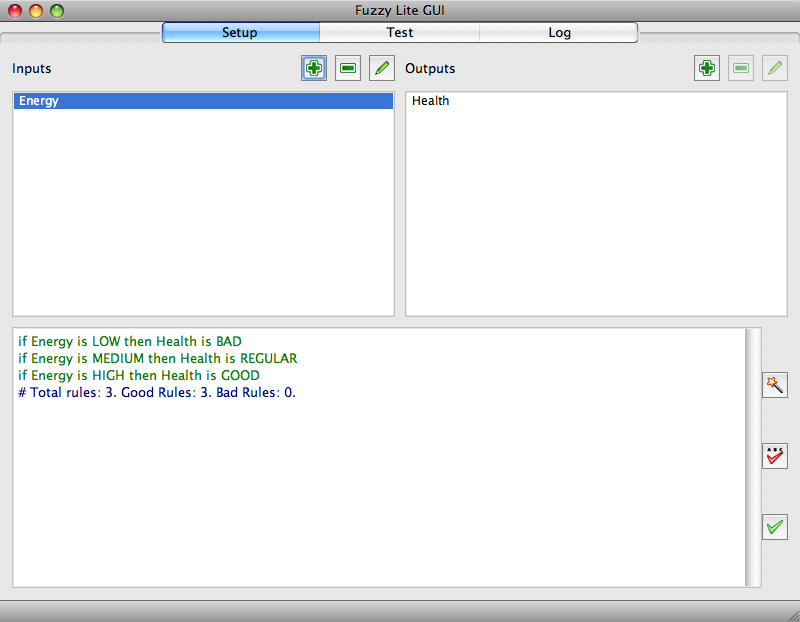
\includegraphics[scale=0.6]{./figures/gui-setup.png}
	\vfill

\clearpage
\section*{GUI Setup}
\addcontentsline{toc}{section}{GUI Test}
	The following figure shows the Setup part of the GUI build for \fl.\\
	\vfill
\noindent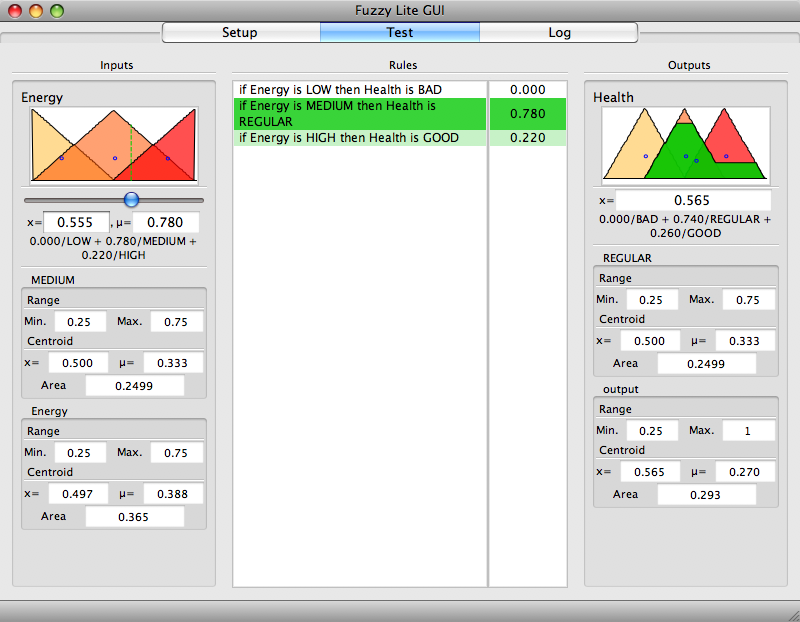
\includegraphics[scale=0.6]{./figures/gui-test.png}
	\vfill

\clearpage
\section*{License of \fl}
\addcontentsline{toc}{section}{License of \fl}
\begin{verbatim}
                             Apache License
                       Version 2.0, January 2004
                    http://www.apache.org/licenses/

TERMS AND CONDITIONS FOR USE, REPRODUCTION, AND DISTRIBUTION

1. Definitions.

  "License" shall mean the terms and conditions for use, reproduction,
  and distribution as defined by Sections 1 through 9 of this document.

  "Licensor" shall mean the copyright owner or entity authorized by
  the copyright owner that is granting the License.

  "Legal Entity" shall mean the union of the acting entity and all
  other entities that control, are controlled by, or are under common
  control with that entity. For the purposes of this definition,
  "control" means (i) the power, direct or indirect, to cause the
  direction or management of such entity, whether by contract or
  otherwise, or (ii) ownership of fifty percent (50%) or more of the
  outstanding shares, or (iii) beneficial ownership of such entity.

  "You" (or "Your") shall mean an individual or Legal Entity
  exercising permissions granted by this License.

  "Source" form shall mean the preferred form for making modifications,
  including but not limited to software source code, documentation
  source, and configuration files.

  "Object" form shall mean any form resulting from mechanical
  transformation or translation of a Source form, including but
  not limited to compiled object code, generated documentation,
  and conversions to other media types.

  "Work" shall mean the work of authorship, whether in Source or
  Object form, made available under the License, as indicated by a
  copyright notice that is included in or attached to the work
  (an example is provided in the Appendix below).

  "Derivative Works" shall mean any work, whether in Source or Object
  form, that is based on (or derived from) the Work and for which the
  editorial revisions, annotations, elaborations, or other modifications
  represent, as a whole, an original work of authorship. For the purposes
  of this License, Derivative Works shall not include works that remain
  separable from, or merely link (or bind by name) to the interfaces of,
  the Work and Derivative Works thereof.

  "Contribution" shall mean any work of authorship, including
  the original version of the Work and any modifications or additions
  to that Work or Derivative Works thereof, that is intentionally
  submitted to Licensor for inclusion in the Work by the copyright owner
  or by an individual or Legal Entity authorized to submit on behalf of
  the copyright owner. For the purposes of this definition, "submitted"
  means any form of electronic, verbal, or written communication sent
  to the Licensor or its representatives, including but not limited to
  communication on electronic mailing lists, source code control systems,
  and issue tracking systems that are managed by, or on behalf of, the
  Licensor for the purpose of discussing and improving the Work, but
  excluding communication that is conspicuously marked or otherwise
  designated in writing by the copyright owner as "Not a Contribution."

  "Contributor" shall mean Licensor and any individual or Legal Entity
  on behalf of whom a Contribution has been received by Licensor and
  subsequently incorporated within the Work.

2. Grant of Copyright License. Subject to the terms and conditions of
  this License, each Contributor hereby grants to You a perpetual,
  worldwide, non-exclusive, no-charge, royalty-free, irrevocable
  copyright license to reproduce, prepare Derivative Works of,
  publicly display, publicly perform, sublicense, and distribute the
  Work and such Derivative Works in Source or Object form.

3. Grant of Patent License. Subject to the terms and conditions of
  this License, each Contributor hereby grants to You a perpetual,
  worldwide, non-exclusive, no-charge, royalty-free, irrevocable
  (except as stated in this section) patent license to make, have made,
  use, offer to sell, sell, import, and otherwise transfer the Work,
  where such license applies only to those patent claims licensable
  by such Contributor that are necessarily infringed by their
  Contribution(s) alone or by combination of their Contribution(s)
  with the Work to which such Contribution(s) was submitted. If You
  institute patent litigation against any entity (including a
  cross-claim or counterclaim in a lawsuit) alleging that the Work
  or a Contribution incorporated within the Work constitutes direct
  or contributory patent infringement, then any patent licenses
  granted to You under this License for that Work shall terminate
  as of the date such litigation is filed.

4. Redistribution. You may reproduce and distribute copies of the
  Work or Derivative Works thereof in any medium, with or without
  modifications, and in Source or Object form, provided that You
  meet the following conditions:

  (a) You must give any other recipients of the Work or
      Derivative Works a copy of this License; and

  (b) You must cause any modified files to carry prominent notices
      stating that You changed the files; and

  (c) You must retain, in the Source form of any Derivative Works
      that You distribute, all copyright, patent, trademark, and
      attribution notices from the Source form of the Work,
      excluding those notices that do not pertain to any part of
      the Derivative Works; and

  (d) If the Work includes a "NOTICE" text file as part of its
      distribution, then any Derivative Works that You distribute must
      include a readable copy of the attribution notices contained
      within such NOTICE file, excluding those notices that do not
      pertain to any part of the Derivative Works, in at least one
      of the following places: within a NOTICE text file distributed
      as part of the Derivative Works; within the Source form or
      documentation, if provided along with the Derivative Works; or,
      within a display generated by the Derivative Works, if and
      wherever such third-party notices normally appear. The contents
      of the NOTICE file are for informational purposes only and
      do not modify the License. You may add Your own attribution
      notices within Derivative Works that You distribute, alongside
      or as an addendum to the NOTICE text from the Work, provided
      that such additional attribution notices cannot be construed
      as modifying the License.

  You may add Your own copyright statement to Your modifications and
  may provide additional or different license terms and conditions
  for use, reproduction, or distribution of Your modifications, or
  for any such Derivative Works as a whole, provided Your use,
  reproduction, and distribution of the Work otherwise complies with
  the conditions stated in this License.

5. Submission of Contributions. Unless You explicitly state otherwise,
  any Contribution intentionally submitted for inclusion in the Work
  by You to the Licensor shall be under the terms and conditions of
  this License, without any additional terms or conditions.
  Notwithstanding the above, nothing herein shall supersede or modify
  the terms of any separate license agreement you may have executed
  with Licensor regarding such Contributions.

6. Trademarks. This License does not grant permission to use the trade
  names, trademarks, service marks, or product names of the Licensor,
  except as required for reasonable and customary use in describing the
  origin of the Work and reproducing the content of the NOTICE file.

7. Disclaimer of Warranty. Unless required by applicable law or
  agreed to in writing, Licensor provides the Work (and each
  Contributor provides its Contributions) on an "AS IS" BASIS,
  WITHOUT WARRANTIES OR CONDITIONS OF ANY KIND, either express or
  implied, including, without limitation, any warranties or conditions
  of TITLE, NON-INFRINGEMENT, MERCHANTABILITY, or FITNESS FOR A
  PARTICULAR PURPOSE. You are solely responsible for determining the
  appropriateness of using or redistributing the Work and assume any
  risks associated with Your exercise of permissions under this License.

8. Limitation of Liability. In no event and under no legal theory,
  whether in tort (including negligence), contract, or otherwise,
  unless required by applicable law (such as deliberate and grossly
  negligent acts) or agreed to in writing, shall any Contributor be
  liable to You for damages, including any direct, indirect, special,
  incidental, or consequential damages of any character arising as a
  result of this License or out of the use or inability to use the
  Work (including but not limited to damages for loss of goodwill,
  work stoppage, computer failure or malfunction, or any and all
  other commercial damages or losses), even if such Contributor
  has been advised of the possibility of such damages.

9. Accepting Warranty or Additional Liability. While redistributing
  the Work or Derivative Works thereof, You may choose to offer,
  and charge a fee for, acceptance of support, warranty, indemnity,
  or other liability obligations and/or rights consistent with this
  License. However, in accepting such obligations, You may act only
  on Your own behalf and on Your sole responsibility, not on behalf
  of any other Contributor, and only if You agree to indemnify,
  defend, and hold each Contributor harmless for any liability
  incurred by, or claims asserted against, such Contributor by reason
  of your accepting any such warranty or additional liability.

END OF TERMS AND CONDITIONS
\end{verbatim}
	
\end{document}
